\documentclass[12pt, a4paper]{ctexart}

%========================================
% 宏包引入
%========================================
\usepackage[margin=2.5cm]{geometry}
\usepackage{amsmath, amssymb, amsthm, mathtools}
\usepackage{xcolor}
\usepackage{graphicx}
\usepackage{tikz}
\usepackage{pgfplots}
\usepackage{tcolorbox}
\usepackage{booktabs}
\usepackage{hyperref}
\usepackage{fancyhdr}
\usepackage{algorithm}
\usepackage{algorithmic}
\usepackage{bm}
\usepackage{listings}
\usepackage{enumerate}

% 设置绘图库
\usetikzlibrary{arrows.meta, positioning, calc, shapes, decorations.pathreplacing, patterns, matrix}
\pgfplotsset{compat=1.18}

%========================================
% 代码高亮设置
%========================================
\lstset{
    language=Python,
    basicstyle=\ttfamily\small,
    keywordstyle=\color{blue}\bfseries,
    commentstyle=\color{gray},
    stringstyle=\color{red},
    numbers=left,
    numberstyle=\tiny\color{gray},
    breaklines=true,
    frame=single,
    backgroundcolor=\color{gray!5}
}

%========================================
% 自定义颜色与环境
%========================================
\definecolor{myblue}{RGB}{0, 102, 204}
\definecolor{myred}{RGB}{204, 0, 0}
\definecolor{mygreen}{RGB}{0, 153, 76}
\definecolor{mypurple}{RGB}{128, 0, 128}
\definecolor{myorange}{RGB}{255, 140, 0}
\definecolor{gpugreen}{RGB}{118, 185, 0}

% 板书环境
\tcbuselibrary{skins, breakable}
\newtcolorbox{blackboard}[1][]{
    colback=gray!10,
    colframe=black!70,
    fonttitle=\bfseries,
    title={#1},
    boxrule=0.5mm,
    sharp corners,
    breakable
}

% 关键结论
\newtcolorbox{keypoint}[1][]{
    colback=myblue!5,
    colframe=myblue,
    fonttitle=\bfseries,
    title={核心要求：#1},
    breakable
}

% GPU要点
\newtcolorbox{gpubox}[1][]{
    colback=gpugreen!10,
    colframe=gpugreen!70!black,
    fonttitle=\bfseries,
    title={GPU视角：#1},
    breakable
}

% 背景说明
\newtcolorbox{mlcontext}[1][]{
    colback=myorange!8,
    colframe=myorange!80!black,
    fonttitle=\bfseries,
    title={大模型背景：#1},
    breakable
}

% 定义与定理
\newtheorem{theorem}{定理}[section]
\newtheorem{lemma}[theorem]{引理}
\newtheorem{definition}[theorem]{定义}

% 自动编号的题目命令
\newcounter{problem}
\newcommand{\problem}[1]{%
    \stepcounter{problem}%
    \section*{第\chinese{problem}题：#1}%
}

%========================================
% 页眉页脚
%========================================
\pagestyle{fancy}
\fancyhf{}
\fancyhead[L]{优化算法：从理论到大规模实践}
\fancyhead[R]{第4周作业}
\fancyfoot[C]{\thepage}

%========================================
% 正文开始
%========================================
\title{第四周作业：\textbf{算法设计范式与GPU化}\\[0.5em]
\Large 分治、动态规划、贪心——及其在大模型中的应用}

\author{优化算法课程}

\begin{document}

\maketitle


%========================================
\problem{主定理与矩阵乘法复杂度}
%========================================

\begin{mlcontext}[Transformer中的矩阵乘法]
大语言模型的注意力机制（Attention）核心操作为矩阵乘法：
$\text{Attention}(Q,K,V) = \text{softmax}\!\left(\frac{QK^\top}{\sqrt{d_k}}\right)V$。
其中 $Q, K, V \in \mathbb{R}^{n \times d}$。分析矩阵乘法算法的时间复杂度对大模型推理效率至关重要。
\end{mlcontext}

\begin{enumerate}[(a)]
    \item 用主定理求解下列递推式的时间复杂度（写出所用的主定理情形）：

    \begin{enumerate}[i.]
        \item $T(n) = 8T(n/2) + O(n^2)$\hfill（朴素矩阵乘法的分治形式）
        \item $T(n) = 7T(n/2) + O(n^2)$\hfill（Strassen算法）
        \item $T(n) = 4T(n/2) + O(n^2)$
        \item $T(n) = 2T(n/2) + O(n\log n)$\hfill（归并排序变体）
    \end{enumerate}

    \item 在Transformer的自注意力中，设序列长度为 $n$，模型维度为 $d$。
    \begin{enumerate}[i.]
        \item 计算 $QK^\top$ 的朴素算法（矩阵乘法）时间复杂度是多少？
        \item 若 $d = O(n)$，朴素算法 vs Strassen算法，哪个渐近更快？给出理由。
        \item 实践中Strassen算法较少用于深度学习，请给出至少一个工程原因。
    \end{enumerate}
\end{enumerate}

%========================================


\problem{动态规划——最长公共子序列（LCS）与代码相似度检测}
%========================================

\begin{mlcontext}[LLM生成代码的抄袭/泄露检测]
大语言模型生成的代码可能与训练数据中的代码高度相似，引发版权和隐私风险。
\textbf{最长公共子序列（LCS）}是衡量两段序列结构相似度的经典方法：
将代码 token 化后，计算生成序列与训练样本的 LCS 长度，
可作为"记忆泄露"（memorization）程度的量化指标。
\end{mlcontext}

\begin{enumerate}[(a)]
    \item 设 $dp[i][j]$ 为序列 $X[1..i]$ 与 $Y[1..j]$ 的最长公共子序列长度。写出：
    \begin{enumerate}[i.]
        \item 状态转移方程（分 $X[i] = Y[j]$ 和 $X[i] \neq Y[j]$ 两种情况讨论）
        \item 边界条件 $dp[i][0]$ 和 $dp[0][j]$
        \item 时间复杂度与空间复杂度
    \end{enumerate}

    \item 设某 LLM 生成的 token 序列为
    $X = [\texttt{def},\; \texttt{sort},\; \texttt{list},\; \texttt{return},\; \texttt{sorted},\; \texttt{list}]$（长度6），
    训练集中的一段代码 token 序列为
    $Y = [\texttt{def},\; \texttt{merge},\; \texttt{sort},\; \texttt{return},\; \texttt{list}]$（长度5）。

    手动填写完整的 DP 表格（$7 \times 6$，含边界行列），给出 LCS 长度。

    \begin{center}
    \begin{tabular}{c|cccccc}
    \toprule
    $dp[i][j]$ & $\varepsilon$ & \texttt{def} & \texttt{merge} & \texttt{sort} & \texttt{return} & \texttt{list} \\
    \midrule
    $\varepsilon$ & 0 & 0 & 0 & 0 & 0 & 0 \\
    \texttt{def} & 0 & & & & & \\
    \texttt{sort} & 0 & & & & & \\
    \texttt{list} & 0 & & & & & \\
    \texttt{return} & 0 & & & & & \\
    \texttt{sorted} & 0 & & & & & \\
    \texttt{list} & 0 & & & & & \\
    \bottomrule
    \end{tabular}
    \end{center}

    回溯找出一个具体的 LCS，并计算相似度指标 $\mathrm{sim} = \dfrac{2\,|\text{LCS}|}{|X| + |Y|}$。

    \item 用\textbf{剪切-粘贴论证法}证明 LCS 的最优子结构：

    \begin{keypoint}[待证命题]
    设 $Z = z_1 z_2 \cdots z_k$ 是 $X[1..m]$ 与 $Y[1..n]$ 的一个 LCS。
    若 $x_m = y_n$，则 $z_k = x_m = y_n$，且 $Z[1..k-1]$ 是 $X[1..m{-}1]$ 与 $Y[1..n{-}1]$ 的 LCS。
    \end{keypoint}

    \textit{提示}：先证 $z_k = x_m$（反证：若不是，可以将 $x_m$ 附加到 $Z$ 末尾得到更长公共子序列）；
    再证 $Z[1..k{-}1]$ 是最优的（若存在更长的公共子序列 $W$，可以粘贴 $x_m$ 得到矛盾）。
\end{enumerate}


%========================================
\problem{分治法——用FFT加速卷积}
%========================================

\begin{mlcontext}[卷积神经网络（CNN）中的卷积加速]
卷积神经网络的核心操作是一维或二维离散卷积。朴素卷积的时间复杂度为 $O(n^2)$，
而利用分治法和快速傅里叶变换（FFT）可将其降至 $O(n\log n)$，
这在处理长序列（如语音、DNA序列）时至关重要。
\end{mlcontext}

\begin{enumerate}[(a)]
    \item 两个长度为 $n$ 的多项式（序列）的卷积朴素算法为 $O(n^2)$。
    Cooley-Tukey FFT 算法采用分治策略，将 DFT 拆分为奇偶两部分：
    \[
        F[k] = F_{\text{even}}[k] + e^{-2\pi i k/n} F_{\text{odd}}[k]
    \]
    写出该算法的递推式，并用主定理求解其时间复杂度。

    \item 对长度 $n = 8$ 的序列，画出 FFT 蝴蝶操作的递归结构示意图（树形图），
    标注每一层的操作数量，并说明：第 $\ell$ 层（$\ell = 1, 2, \ldots, \log_2 n$）共有多少个独立的蝴蝶操作？

    \item 在 GPU 上并行执行 FFT 时：
    \begin{enumerate}[i.]
        \item 每一层的蝴蝶操作可以完全并行，假设 GPU 有足够的并行核心（$\geq n/2$），
        分析 GPU 上 FFT 的并行时间复杂度（按层数计）。
        \item 相比 CPU 上 $O(n\log n)$ 的顺序时间，GPU 上的加速比是多少？
        \item 用FFT加速CNN卷积时，实际并行效率受哪些因素影响？请列举两点。
    \end{enumerate}
\end{enumerate}

%========================================

%========================================
\problem{动态规划——矩阵链乘法与最优括号化}
%========================================

\begin{mlcontext}[Transformer中的多矩阵乘法顺序优化]
Transformer推理时，一个注意力头的计算为 $((QK^\top)V)W_O$，
涉及多个矩阵连乘。不同的括号化方式（计算顺序）会导致截然不同的计算量。
对矩阵链乘法顺序进行优化，可显著降低推理时间。
\end{mlcontext}

\begin{enumerate}[(a)]
    \item 写出矩阵链乘法的 DP 状态定义和转移方程：
    设 $m[i,j]$ 为计算矩阵 $A_i A_{i+1} \cdots A_j$ 所需的最少标量乘法次数，
    写出 $m[i,j]$ 的递推式（$i < j$ 时），以及时间复杂度。

    \item 给定如下4个矩阵（维度模拟Transformer注意力计算）：
    \[
        A_1 \in \mathbb{R}^{64 \times 512}, \quad
        A_2 \in \mathbb{R}^{512 \times 64}, \quad
        A_3 \in \mathbb{R}^{64 \times 512}, \quad
        A_4 \in \mathbb{R}^{512 \times 1}
    \]
    \begin{enumerate}[i.]
        \item 用 DP 方法求计算 $A_1 A_2 A_3 A_4$ 的\textbf{最优括号化方式}及最少标量乘法次数。
        请填写 $m[i,j]$ 的完整表格。
        \item 列举所有可能的括号化方式中，\textbf{最差}的括号化方式需要多少次标量乘法？
        与最优方案相差多少倍？
    \end{enumerate}
\end{enumerate}

%========================================
\problem{状态压缩DP——Beam Search路径规划}
%========================================

\begin{mlcontext}[语言模型解码：Beam Search vs 贪心解码]
语言模型自回归生成时，每步从词表 $V$ 中选一个token。
\textbf{贪心解码}每步选概率最高的token；\textbf{Beam Search}保留 $B$ 条候选路径，
以期找到全局更优的序列。理解这两种解码策略的本质，需要动态规划的视角。
\end{mlcontext}

\begin{enumerate}[(a)]
    \item 考虑一个简化问题：词表大小为 $n$，生成长度为 $T$ 的序列，
    每步的对数概率为 $\log p(\text{token}_t | \text{context})$。
    \begin{enumerate}[i.]
        \item 将"找最大对数概率序列"形式化为DP问题，定义状态和转移方程。
        \item 暴力枚举所有长度为 $T$ 的序列的时间复杂度是多少？DP能否将其降低？为什么？
        （提示：注意这里的语言模型是自回归的，即 $p(x_t | x_{<t})$ 依赖全部历史。）
    \end{enumerate}

    \item 考虑如下反例：词表 $V = \{A, B, C\}$，生成长度 $T=3$，各步概率如下表：

    \begin{center}
    \begin{tabular}{c|ccc|ccc|ccc}
    \toprule
    步骤 & \multicolumn{3}{c|}{第1步} & \multicolumn{3}{c|}{第2步（上步选A）} & \multicolumn{3}{c}{第3步（前两步AB）} \\
    \midrule
    Token & A & B & C & A & B & C & A & B & C \\
    概率   & 0.5 & 0.3 & 0.2 & 0.1 & 0.8 & 0.1 & 0.35 & 0.33 & 0.32 \\
    \midrule
    & \multicolumn{3}{c|}{} & \multicolumn{3}{c|}{第2步（上步选B）} & \multicolumn{3}{c}{第3步（前两步BA）} \\
    \midrule
    Token & & & & A & B & C & A & B & C \\
    概率   & & & & 0.6 & 0.3 & 0.1 & 0.1 & 0.8 & 0.1 \\
    \bottomrule
    \end{tabular}
    \end{center}

    \begin{enumerate}[i.]
        \item 贪心解码给出的序列是什么？总概率是多少？
        \item 通过枚举，找到概率最高的序列（长度3），证明贪心解码\textbf{不一定}给出全局最优解。
    \end{enumerate}

    \item 经典\textbf{TSP状压DP}（旅行商问题）：$n$ 个城市，$dp[S][v]$ 表示
    从城市0出发，已访问城市集合为 $S$，当前在城市 $v$ 的最短路径长度。
    \begin{enumerate}[i.]
        \item 写出 $dp[S][v]$ 的状态转移方程。
        \item 状态总数和总时间复杂度各是多少？
        \item 若每个城市代表一个候选解码步骤，这与Beam Search有何结构上的相似性？
        简要说明（3句话以内）。
    \end{enumerate}
\end{enumerate}



%========================================



\problem{KV Cache 页分配——前缀共享下的树形背包DP}
%========================================
 
\begin{mlcontext}[vLLM 的 PagedAttention 与前缀共享]
大模型推理引擎（如 vLLM）使用 \textbf{PagedAttention}：
将 KV Cache 分成固定大小的\textbf{物理页}（block），按需分配给各请求。
当多个请求共享\textbf{相同的前缀}（如相同的 system prompt）时，
共享前缀对应的 KV Cache 页只需存储\textbf{一份}，多个请求可共用——这称为
\textbf{prefix sharing}（前缀共享），是 vLLM 的关键优化之一。
在物理页总量有限时，如何选择服务哪些请求、利用前缀共享节省页数，
可以建模为一个\textbf{树形依赖背包问题}。
\end{mlcontext}
 
\begin{blackboard}[问题形式化]
系统中有若干推理请求，它们的 prompt 前缀关系构成一棵\textbf{前缀树}（trie）。
树中的每个\textbf{内部节点}代表一段共享前缀，占用若干物理页；
每个\textbf{叶节点}代表一个具体请求的独有后缀部分。
 
\begin{itemize}
    \item 每个节点 $v$ 有\textbf{页开销} $c(v)$（存储该段 KV Cache 所需的物理页数）
    \item 每个\textbf{叶节点}（请求）有\textbf{服务收益} $w(v)$（如用户优先级、预期收入）；
    内部节点的收益为 0（共享前缀本身不产生收益，仅为请求服务）
    \item \textbf{依赖约束}：要服务某个请求（叶节点），必须分配从根到该叶的\textbf{整条路径}上所有节点的页
    \item 前缀共享：若两个请求共享某段前缀，该前缀的页\textbf{只需分配一次}
\end{itemize}
 
目标：在总物理页预算 $P$ 内，选择一些请求服务，使总收益最大化。
\end{blackboard}
 
\begin{enumerate}[(a)]
    \item \textbf{树形DP状态定义。}
    设 $dp[v][j]$ 为以 $v$ 为根的子树中，分配 $j$ 个物理页时可获得的最大收益。
    注意：\textbf{选择子树中的任何叶节点，都必须先为节点 $v$ 本身分配 $c(v)$ 页}。
 
    \begin{enumerate}[i.]
        \item 写出叶节点（请求节点）的边界条件：
        \[
        dp[v][j] = \begin{cases} ? & \text{if } j \geq c(v) \\ ? & \text{if } j < c(v) \end{cases}
        \]
        \item 写出内部节点 $v$（子节点集合为 $\text{ch}(v) = \{u_1, u_2, \ldots\}$）的状态转移方程。
 
        \textit{提示}：先为 $v$ 本身保留 $c(v)$ 页，剩余 $j - c(v)$ 页在各子树间分配。
        子树之间的页分配相互独立，等价于对子树做\textbf{分组背包合并}：
        依次合并每个子树的 DP 表。
    \end{enumerate}
 
    \item \textbf{手算例子。}
    下图为一个前缀树，共5个请求（叶节点 $R_1$--$R_5$）。
    每个节点标注为 $[w, c]$（收益, 页开销）。物理页预算 $P = 7$。
 
\begin{center}
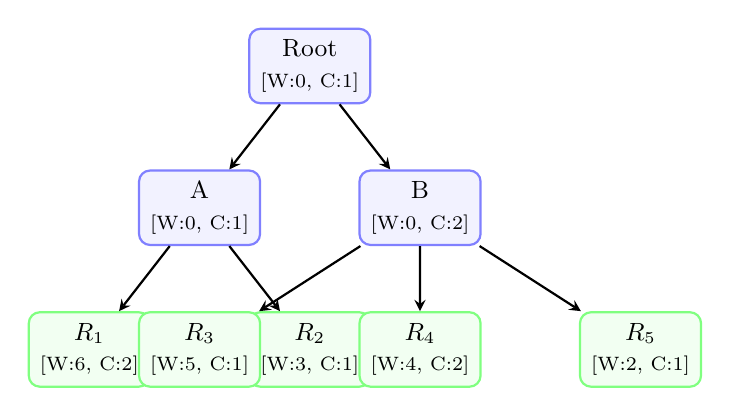
\begin{tikzpicture}[
    % 基础样式定义
    every node/.style={draw, rounded corners, font=\small, minimum height=0.9cm, inner sep=4pt, align=center},
    % 内部节点（共享前缀）
    internal/.style={fill=blue!5, draw=blue!50, thick},
    % 叶子节点（请求）
    request/.style={fill=green!5, draw=green!50, thick},
    level distance=1.8cm,
    sibling distance=2.8cm,
    edge from parent/.style={draw, -stealth, thick}
]

% 根节点
\node[internal] {Root \\ \scriptsize [W:0, C:1]}
    child { node[internal] {A \\ \scriptsize [W:0, C:1]}
        child { node[request] {$R_1$ \\ \scriptsize [W:6, C:2]} }
        child { node[request] {$R_2$ \\ \scriptsize [W:3, C:1]} }
    }
    child { node[internal] {B \\ \scriptsize [W:0, C:2]}
        child { node[request] {$R_3$ \\ \scriptsize [W:5, C:1]} }
        child { node[request] {$R_4$ \\ \scriptsize [W:4, C:2]} }
        child { node[request] {$R_5$ \\ \scriptsize [W:2, C:1]} }
    };

\end{tikzpicture}
\end{center}
 
    例如，服务请求 $R_1$ 需要分配路径 root $\to A \to R_1$ 共 $1 + 1 + 2 = 4$ 页；
    若同时服务 $R_1$ 和 $R_2$，共享 root 和 $A$ 的页，总共只需 $1 + 1 + 2 + 1 = 5$ 页。
 
    \begin{enumerate}[i.]
        \item 自底向上计算每个节点的 $dp[v][j]$ 表。
        先算叶节点 $R_1$--$R_5$，再合并算内部节点 $A$、$B$，最后算 root。
        \item 在预算 $P = 7$ 下，最优方案服务哪些请求？最大总收益是多少？
        \item 验证前缀共享带来的节省：
        若不共享前缀（每个请求独立分配从根到叶的全部页），
        服务同样的请求集合需要多少页？节省了多少？
    \end{enumerate}
 
    \item \textbf{复杂度分析。}
    \begin{enumerate}[i.]
        \item 合并两个子树的 DP 表（大小分别为 $s_1$ 和 $s_2$）需要 $O(s_1 \cdot s_2)$ 时间。
        说明整棵树的总合并时间为 $O(nP^2)$，其中 $n$ 为节点数。
        \item 在实际 LLM serving 中，$n$ 可达数百（请求数 + 共享前缀数），$P$ 可达数千（GPU显存页数）。
        $O(nP^2)$ 是否实际可行？若不可行，提出一种降低复杂度的思路。
        （提示：如果大部分子树的 $dp$ 表是稀疏的，可以怎样优化？）
    \end{enumerate}
\end{enumerate}
 


%========================================
\problem{0-1背包的FPTAS——大模型推理预算分配}
%========================================
 
\begin{mlcontext}[LLM Serving 中的请求选择]
在大规模 LLM 服务中，当系统过载时，需要从等待队列中选择一批请求处理，
使得在有限的计算预算（GPU 算力或 KV Cache 容量）内，总服务质量最高。
每个请求的计算开销（token 数）和优先级（SLA 等级、付费用户权重）不同，
这本质上是一个\textbf{0-1背包问题}。精确 DP 的复杂度 $O(nW)$ 在预算 $W$ 很大时不可行，
而 \textbf{FPTAS}（全多项式时间近似方案）通过值域缩放，
能在 $O(n^2/\varepsilon)$ 时间内找到 $(1-\varepsilon)$ 近似解。
\end{mlcontext}
 
\begin{enumerate}[(a)]
    \item \textbf{伪多项式时间与NP难的关系。}
    0-1背包的精确 DP 复杂度为 $O(nW)$。
    \begin{enumerate}[i.]
        \item 若输入中 $W$ 用二进制表示，其编码长度为 $\lceil \log_2 W \rceil$ 位。
        说明 $O(nW) = O(n \cdot 2^{\lceil \log_2 W \rceil})$，即对输入编码长度而言是\textbf{指数级}的。
        这就是"伪多项式时间"的含义。
        \item 0-1背包是\textbf{弱NP难}问题。解释"弱NP难"与"强NP难"的区别，
        并各举一个例子。
    \end{enumerate}
 
    \item \textbf{FPTAS 算法描述。}
    给定 $\varepsilon > 0$，FPTAS 通过以下步骤将0-1背包转化为多项式时间可解的问题：
 
    \begin{enumerate}[i.]
        \item 令 $V_{\max} = \max_i v_i$，缩放因子 $K = \dfrac{\varepsilon \cdot V_{\max}}{n}$。
        对每个物品计算缩放后的价值 $v'_i = \left\lfloor \dfrac{v_i}{K} \right\rfloor$。
        说明每个 $v'_i$ 的取值范围（用 $n, \varepsilon$ 表示上界）。
        \item 对缩放后的问题，运行\textbf{最小重量 DP}：
        $dp[v]$ 表示恰好达到总缩放价值 $v$ 时的最小总重量。
        写出 $dp[v]$ 的状态转移方程和初始条件。
        \item DP 表的大小（$v$ 的上界）是多少？（用 $n, \varepsilon$ 表示）
        总时间复杂度是多少？验证这是关于 $n$ 和 $1/\varepsilon$ 的多项式。
    \end{enumerate}
 
    \item \textbf{近似比证明。}
    设 $\mathrm{OPT}$ 为精确最优值，$\mathrm{ALG}$ 为 FPTAS 的输出值。
 
    \begin{keypoint}[待证命题]
    $\mathrm{ALG} \geq (1 - \varepsilon)\,\mathrm{OPT}$。
    \end{keypoint}
 
    \textit{提示}：
    \begin{enumerate}[i.]
        \item 设 $S^*$ 为最优解的物品集合。说明每个物品取整损失 $v_i - K \cdot v'_i < K$，
        因此总损失 $\mathrm{OPT} - K \cdot \sum_{i \in S^*} v'_i < n \cdot K = \varepsilon \cdot V_{\max}$。
        \item 说明 $V_{\max} \leq \mathrm{OPT}$（最优解至少包含一个物品），
        从而总损失 $< \varepsilon \cdot \mathrm{OPT}$。
        \item 设 FPTAS 的解为 $S'$，在缩放问题中 $S'$ 是最优的。
        综合以上两步，完成证明：
        $\mathrm{ALG} \geq K \cdot \sum_{i \in S'} v'_i \geq K \cdot \sum_{i \in S^*} v'_i \geq (1-\varepsilon)\,\mathrm{OPT}$。
    \end{enumerate}
 
    \item \textbf{数值手算。}
    5个推理请求，计算预算 $W = 11$：
 
    \begin{center}
    \begin{tabular}{ccccc}
    \toprule
    请求 $i$ & 计算开销 $w_i$ & 服务收益 $v_i$ & $v_i / K$ & 缩放后 $v'_i$ \\
    \midrule
    1 & 5 & 35  & & \\
    2 & 2 & 155 & & \\
    3 & 6 & 50  & & \\
    4 & 4 & 250 & & \\
    5 & 2 & 30  & & \\
    \bottomrule
    \end{tabular}
    \end{center}
 
    取 $\varepsilon = 0.4$。
    \begin{enumerate}[i.]
        \item 计算 $V_{\max}$、$K$、以及每个物品的缩放价值 $v'_i$（填入上表）。
        DP 表的大小（$v'$ 的上界 $\sum_i v'_i$）是多少？
        \item 运行缩放后的最小重量 DP。
        \textit{提示}：不需要填写全部表格，只需追踪 $dp[v']$ 中能够被 $W=11$ 容纳的那些状态。
        找到 FPTAS 的近似解：选了哪些请求？近似总收益 $\mathrm{ALG}$ 是多少？
        \item 用暴力枚举（$2^5 = 32$ 种子集）求出精确最优值 $\mathrm{OPT}$ 及最优方案。
        计算 $\mathrm{ALG}/\mathrm{OPT}$，验证是否 $\geq 1 - \varepsilon = 0.6$。
        \item 观察：FPTAS 的解与精确最优解有何不同？
        造成这种差异的原因是什么？
        （提示：比较两个方案在缩放后的价值 $\sum v'_i$ 和实际价值 $\sum v_i$。）
    \end{enumerate}
\end{enumerate}
 

%========================================
\problem{贪心算法——Huffman编码与词表压缩}
%========================================

\begin{mlcontext}[LLM词表压缩与Zipf定律]
大语言模型的词表通常包含数万个token，且其频率分布遵循\textbf{Zipf定律}（极度不均匀）：
少数高频词出现极为频繁，大量低频词极少出现。
Huffman编码可利用这种不均匀性压缩存储空间，是模型量化与压缩的理论基础之一。
\end{mlcontext}

\begin{enumerate}[(a)]
    \item 给定6个高频token及其在语料中出现的相对频率（单位：千次）：

    \begin{center}
    \begin{tabular}{ccccccc}
    \toprule
    Token & \texttt{the} & \texttt{a} & \texttt{is} & \texttt{of} & \texttt{in} & \texttt{to} \\
    \midrule
    频率 & 45 & 13 & 12 & 16 & 9 & 5 \\
    \bottomrule
    \end{tabular}
    \end{center}

    按 Huffman 算法构造最优前缀编码树，画出 Huffman 树（标注每条边的0/1），
    并写出每个token的编码。

    \item 计算：
    \begin{enumerate}[i.]
        \item Huffman编码的\textbf{平均编码长度}（按频率加权）；
        \item 若使用等长编码（$\lceil \log_2 6 \rceil$ 位），平均编码长度是多少？
        \item Huffman编码相比等长编码节省了多少比例的空间？
    \end{enumerate}

    \item 用\textbf{交换论证法（exchange argument）}证明 Huffman 算法的贪心选择性质：

    \begin{keypoint}[待证命题]
    在最优前缀编码树中，频率最低的两个符号一定是兄弟节点（位于树的最深层）。
    \end{keypoint}

    \textit{提示}：假设最优树中频率最低的符号 $x, y$ 不是深度最大的兄弟节点，
    构造一棵交换后的树，证明交换不会增加（反而可能减少）平均编码长度，从而导出矛盾。
\end{enumerate}




\problem{贪心调度——GPU推理请求的最小最大延迟}
%========================================

\begin{mlcontext}[大模型推理服务的请求调度]
在生产环境中，推理服务器（如 vLLM、TensorRT-LLM）同时接收大量用户请求，
每个请求有不同的处理时间（由序列长度决定）和截止时间（用户的SLA要求）。
合理调度请求顺序，可以最小化用户的最大等待超时时间。
\end{mlcontext}

\begin{enumerate}[(a)]
    \item 设有 $n$ 个推理请求，请求 $i$ 的处理时间为 $t_i$，截止时间为 $d_i$。
    所有请求在时刻0均已到达，每次只处理一个请求（单GPU）。
    定义请求 $i$ 的\textbf{延迟}为 $L_i = C_i - d_i$，其中 $C_i$ 为其完成时刻；
    若 $C_i \leq d_i$ 则延迟为负（未超时）。目标是最小化最大延迟 $L_{\max} = \max_i L_i$。

    证明：\textbf{最早截止时间优先（EDF）策略}（按 $d_i$ 升序调度）最小化 $L_{\max}$。

    \textit{提示}：用交换论证法——若某调度 $\sigma$ 中存在相邻两个请求 $i, j$ 满足 $d_i > d_j$
    但 $i$ 排在 $j$ 之前，证明交换它们不会增大 $L_{\max}$。

    \item 对如下4个推理请求，按EDF策略调度，计算每个请求的完成时刻、延迟，
    以及最大延迟 $L_{\max}$：

    \begin{center}
    \begin{tabular}{ccccc}
    \toprule
    请求 & $t_i$（处理时间） & $d_i$（截止时间） & $C_i$（完成时刻） & $L_i$（延迟） \\
    \midrule
    1 & 2 & 4 & & \\
    2 & 1 & 2 & & \\
    3 & 3 & 7 & & \\
    4 & 2 & 5 & & \\
    \bottomrule
    \end{tabular}
    \end{center}
\end{enumerate}

%========================================


\problem{FlashAttention——分块、IO复杂度与在线softmax}
%========================================

\begin{mlcontext}[FlashAttention：IO感知的注意力算法]
标准注意力需要将 $n \times n$ 的注意力矩阵 $S = QK^\top/\sqrt{d}$ 物化到 GPU 的
\textbf{HBM}（高带宽显存，容量大但带宽有限），再读回做 softmax 和乘 $V$。
当序列长度 $n$ 很大时，这 $O(n^2)$ 的 HBM 读写成为瓶颈。
\textbf{FlashAttention}（Dao et al., 2022）采用分块策略：
将 $Q, K, V$ 按序列维度分成大小为 $B$ 的块，在片上 \textbf{SRAM}（容量小但速度极快）中
逐块计算注意力，并利用\textbf{在线 softmax} 技巧实时修正归一化，
从而\textbf{无需物化完整注意力矩阵}，将额外显存从 $O(n^2)$ 降至 $O(n)$。
\end{mlcontext}

\begin{enumerate}[(a)]
    \item \textbf{分块策略与显存分析。}
    标准注意力的中间结果 $S \in \mathbb{R}^{n \times n}$ 需要 $O(n^2)$ 显存。
    FlashAttention 将 $Q$ 分成 $T_Q = \lceil n/B_r \rceil$ 个块，
    $K, V$ 分成 $T_{KV} = \lceil n/B_c \rceil$ 个块，
    每次在 SRAM 中只存储一个 $B_r \times B_c$ 的局部注意力块。

    \begin{enumerate}[i.]
        \item 每次 SRAM 中需要存储的数据包括：
        一个 $Q$ 块（$B_r \times d$）、一个 $K$ 块（$B_c \times d$）、
        一个 $V$ 块（$B_c \times d$）、局部注意力块（$B_r \times B_c$）、
        以及输出累加器（$B_r \times d$）。
        写出 SRAM 占用量关于 $B_r, B_c, d$ 的表达式。
        若 $B_r = B_c = B$，SRAM 大小 $M$ 需要满足什么条件？
        \item 解释为何 FlashAttention 的\textbf{额外显存}（不含输入 $Q, K, V$ 和最终输出 $O$）
        只有 $O(n)$ 而非 $O(n^2)$。
        这 $O(n)$ 具体存储的是什么？
    \end{enumerate}

    \item \textbf{IO 复杂度分析。}
    FlashAttention 的核心收益在于减少 HBM 读写次数。

    \begin{enumerate}[i.]
        \item 标准注意力需要：(1) 从 HBM 读 $Q, K$ 计算 $S = QK^\top$，将 $S$ 写回 HBM；
        (2) 从 HBM 读 $S$ 做 softmax，将 $P = \text{softmax}(S)$ 写回；
        (3) 从 HBM 读 $P, V$ 计算输出。
        写出标准注意力的总 HBM 读写量（用 $n, d$ 表示，忽略常数）。
        \item FlashAttention 的外层循环遍历 $T_{KV}$ 个 $KV$ 块，
        内层循环遍历 $T_Q$ 个 $Q$ 块。每次内层迭代从 HBM 读取一个 $Q$ 块和对应的输出块，
        写回更新后的输出块。每次外层迭代读取一个 $KV$ 块。
        写出总 HBM 读写量关于 $n, d, B_r, B_c$ 的表达式。
        \item 令 $B_r = B_c = B = \Theta(M/d)$（SRAM 约束），
        将 HBM 读写量用 $n, d, M$ 表示。
        当 $M = \Theta(nd)$（SRAM 足够大）时，IO 量为多少？
        与标准注意力的 $O(n^2 d)$ 相比改善了多少？
    \end{enumerate}

    \item \textbf{在线 softmax 与经典分治的对比。}

    分块计算 $\text{softmax}(QK^\top) \cdot V$ 的核心难点在于：
    softmax 需要对第 $i$ 个 query 的\textbf{全部} $n$ 个 key 的得分做归一化，
    但每个块只看到 $B_c$ 个 key。

    \begin{enumerate}[i.]
        \item 设前 $j$ 个 $K$ 块处理完后，第 $i$ 个 query 已累积的局部结果为
        $\tilde{o}_i^{(j)} = \sum_{k \leq jB_c} e^{s_{ik} - m_i^{(j)}} v_k$
        和对应的 log-sum-exp $L_i^{(j)} = \log \sum_{k \leq jB_c} e^{s_{ik} - m_i^{(j)}}$，
        其中 $m_i^{(j)}$ 为当前已见得分的最大值。
        当处理第 $j{+}1$ 个 $K$ 块后，新的最大值可能更新为 $m_i^{(j+1)} > m_i^{(j)}$。
        写出 $\tilde{o}_i^{(j+1)}$ 的更新公式（需要对旧的 $\tilde{o}_i^{(j)}$ 做什么修正？）。
        \item 经典分治（如 Merge Sort）的子问题\textbf{独立}求解后合并，合并时不修改子问题的内部结果。
        FlashAttention 的在线 softmax 与此有何本质区别？
        这种区别对 GPU 并行性有什么影响？
    \end{enumerate}
\end{enumerate}

\end{document}
